\documentclass[cjk,dvipdfmx,10pt,compress,%
hyperref={bookmarks=true,bookmarksnumbered=true,bookmarksopen=false,%
colorlinks=false,%
pdftitle={第 103 回 関西 Debian 勉強会},%
pdfauthor={岩松 信洋},%
%pdfinstitute={関西 Debian 勉強会},%
pdfsubject={資料},%
}]{beamer}

\title{第 103 関西 Debian 勉強会 \\in 関西オープンソース 2015}
\subtitle{Debian と arm64サポート}
\author[岩松 信洋]{{岩松 信洋}}
\institute[Debian JP]{{\normalsize\tt 関西 Debian 勉強会}}
\date{{\small 2015 年 11 月 7 日}}

%\usepackage{amsmath}
%\usepackage{amssymb}
\usepackage{graphicx}
\usepackage{moreverb}
\usepackage[varg]{txfonts}
\AtBeginDvi{\special{pdf:tounicode EUC-UCS2}}
\usetheme{Kyoto}
\def\museincludegraphics{%
  \begingroup
  \catcode`\|=0
  \catcode`\\=12
  \catcode`\#=12
  \includegraphics[width=0.9\textwidth]}
%\renewcommand{\familydefault}{\sfdefault}
%\renewcommand{\kanjifamilydefault}{\sfdefault}
\begin{document}
\settitleslide
\begin{frame}
\titlepage
\end{frame}
\setdefaultslide

\begin{frame}[fragile]
  \frametitle{Disclaimer}
  \begin{itemize}
  \item 疑問、質問、ツッコミ、茶々、\alert{大歓迎}
  \item その場でインタラクティブにどうぞ
  \item ハッシュタグ \#kansaidebian
  \end{itemize}
\end{frame}

\begin{frame}[fragile]
  \frametitle{自己紹介}
  \begin{itemize}
  \item 岩松 信洋
  \item Debian Project 公式開発者
  \item Bluetooth周り、Erlang、Mozc、Macbook、OpenCV、NFC
  \item 2015年度 Debian JP Project Leader
  \item Linux kernel、U-Boot、Xfce、etc
  \item 実家は京都
  \item 普段は埼玉にいます(さいたま!さいたま!)
  \end{itemize}
\end{frame}

\begin{frame}[fragile]
\frametitle{Agenda}

\tableofcontents

\end{frame}

\section{最近の Debian 関係のイベント}

\takahashi[40]{最近の Debian\\関係のイベント}

\begin{frame}[fragile]
  \frametitle{第102回関西Debian勉強会}
  \begin{itemize}
  \item 日時: 9月27日(日)
  \item 場所: 福島区民センター
  \end{itemize}
  \begin{block}{内容}
    \begin{itemize}
    \item ドイツ、ハイデルベルクで開催されたDebconf15へいってきました \\
          (矢吹幸治さん)
    \end{itemize}
  \end{block}
\end{frame}

\begin{frame}[fragile]
  \frametitle{第131回東京エリアDebian勉強会}
  \begin{itemize}
  \item 日時: 10月18日(日)
  \item 場所: イベント&コミュニティスペース dots.
  \end{itemize}
  \begin{block}{内容}
    \begin{itemize}
    \item 毎日使える IPv6 ネットワークの構築 \\ (Rogerさん)
    \end{itemize}
  \end{block}
\end{frame}

\begin{frame}[fragile]
  \frametitle{第132回東京エリアDebian勉強会 in OSC 2015 Tokyo/Fall}
  \begin{itemize}
  \item 日時: 10月24日(土)
  \item 場所: 明星大学 日野キャンパス 28号館 
  \end{itemize}
  \begin{block}{内容}
    \begin{itemize}
    \item ブース・展示
    \begin{center}
    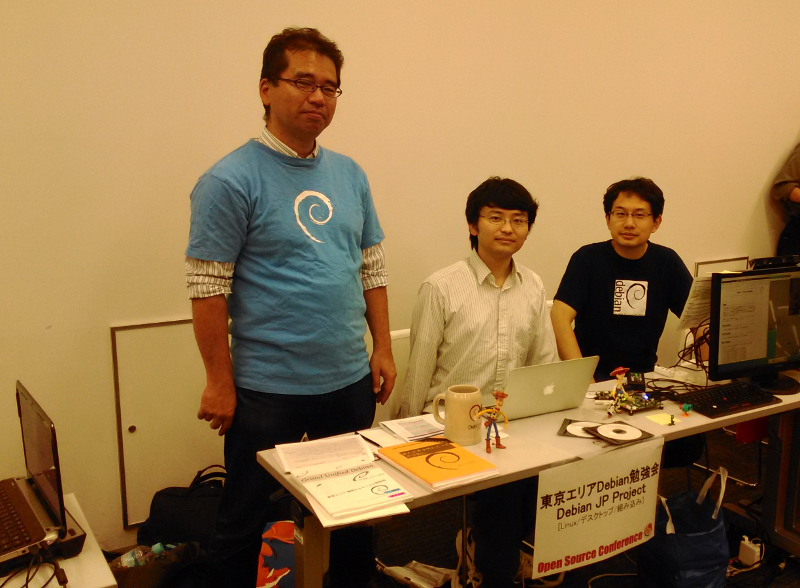
\includegraphics[width=0.4\hsize]{image201511/osc2015-tokyo-fall.png}
    \end{center}
    \item Debian と systemdについて (岩松 信洋)
    \end{itemize}
  \end{block}
\end{frame}

\section{最近のDebian に関する話題}
\takahashi[50]{DebianのDebianに関する話題}

\begin{frame}[fragile]
  \frametitle{最近(ここ一年) のDebian に関する話題}

  \begin{itemize}
\item 2015-04-15 2015年度 Debian  Project Leader が Neil McGovern 氏に
\item 2015-04-25 Debian 8 Jessie リリース
\item 2015-06-06 Debian 8: 8.1 リリース
\item 2015-08-05 DebConf15 開催
\item 2015-09-05 Debian 8: 8.2 リリース
\item 2015 09-05 Updated Debian 7: 7.9 リリース
\item LTS 開始
\item GCC 5 移行
  \end{itemize}

\end{frame}




\section{Debian と arm64サポート}
\takahashi[50]{Debian と arm64サポート}

\begin{frame}[fragile]
  \frametitle{arm64}
  \begin{itemize}
  \item Debian 8.0 から arm64 サポートが入った
  \item Debian でサポートする ARM アーキテクチャ
 \begin{itemize}
  \item armel\\
  32bit / litte endian / ARMv5t

  古いNAS(QNAP、Buffalo、etc)やルータで使用されている ARM SoCで利用可能。

  \item armhf\\
  32bit / litte endian / ARMv7 + VFP3(浮動小数点演算ユニット)

  Raspberry Pi \textcolor{red}{2} などで利用可能。

  \item arm64 $\leftarrow$ \textcolor{red}{New!}

  \end{itemize}

  \item Raspbian

  \begin{itemize}
  \item 32bit / litte endian / ARMv6 + VFP2(浮動小数点演算ユニット)

       Raspberry Pi \textcolor{red}{1} などで利用可能。
  \item Raspbian in not Debian

  \end{itemize}

  \end{itemize}

\end{frame}


\begin{frame}[fragile]
  \frametitle{arm64}
  \begin{itemize}
  \item ARMv8 (ARM Version 8)
  \end{itemize}
  \begin{center}
  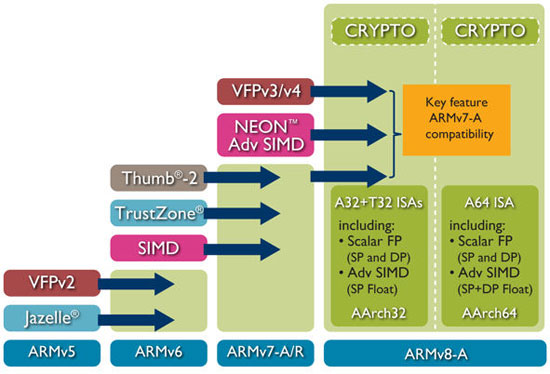
\includegraphics[width=0.7\hsize]{image201511/V5_to_V8_Architecture.jpg}
  \end{center}
\end{frame}

\begin{frame}[fragile]
  \frametitle{arm64}

\begin{minipage}{0.7\hsize}
\begin{itemize}
\item ARMv8 (ARM Version 8)
\item オリジナルコアとしてはCortex-A57、ARM Cortex-A53とCortex-A72がある
\item 正式名称はAArch64
\item Linux kernel では わかりにくいということで arm64 に\\
\url{https://lkml.org/lkml/2012/7/15/133}
\item Debian もこれに追従して arm64 とした
\item コンパイラなどのトリプレットは aarch64-linux-gnu 
\item GCC の定義は \_\_aarch64\_\_ 
\end{itemize}
\end{minipage}

\end{frame}

\begin{frame}[fragile]
  \frametitle{arm64}

  \begin{center}
  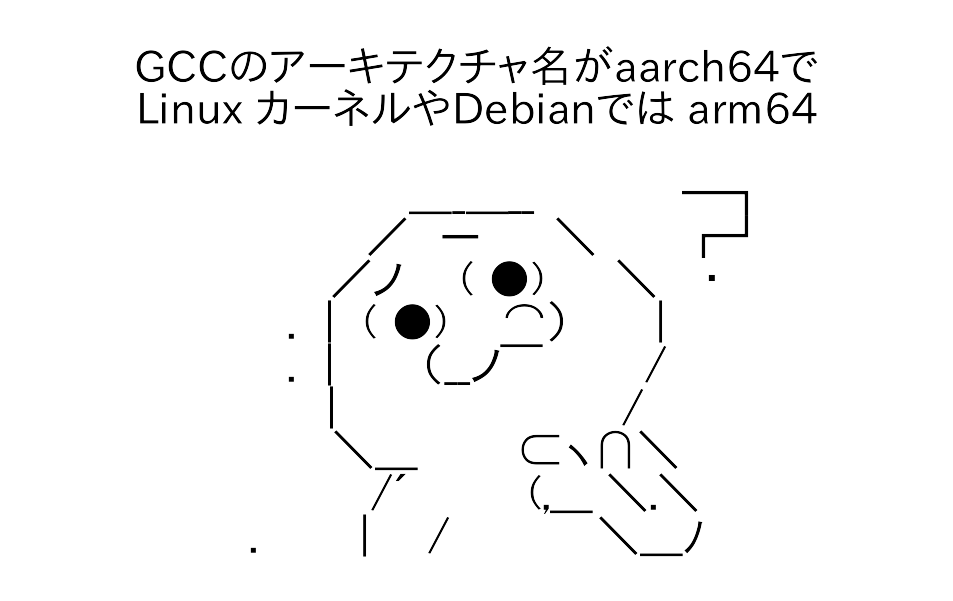
\includegraphics[width=0.8\hsize]{image201511/yaruoAA.png}
  \end{center}
\end{frame}

\begin{frame}[fragile]
  \frametitle{Debian ARM 開発体制}

  \begin{itemize}
  \item 2012 年から開発開始
  \item 開発に参加している多くのDebian Developer が Linaro 所属

   Steve McIntyre、 Wookey、Riku Voipio など

  \item GCC/binutils:

    Matthias Klose (GCC Upstream, Ubuntu Developer でもある)
  \item libc:
    
    Aurelien Jarno、libc メンテナチーム
  \item Linux kernel:

    Ben Hutchings(Linux 3.2 LTS メンテナ)、Ian Campbell(Xen、Allwinner SoCs 関
連)、その他大勢

  % \item Linaro の成果が Debian と Ubuntuに回るサイクルができている

  \end{itemize}
\end{frame}

\begin{frame}[fragile]
  \frametitle{Debian ARM 開発体制}

  \begin{itemize}
  \item Buildd: Applied Micro の X-gene を使ったサーバで運用中
     \url{https://buildd.debian.org/status/architecture.php?a=arm64&suite=sid}
  \item SoC: X-C1 / 2.4Ghz / 8コア 独自コア

  \begin{center}
  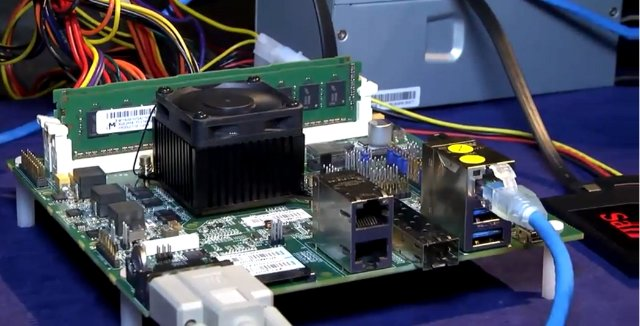
\includegraphics[width=0.7\hsize]{image201511/x-gene.jpg}
  \end{center}

  \end{itemize}
\end{frame}


%FIXME not find image201511/graph-week-big.png
%\begin{frame}[fragile]
%  \frametitle{Debian ARM 開発体制}
%
%  \begin{center}
%  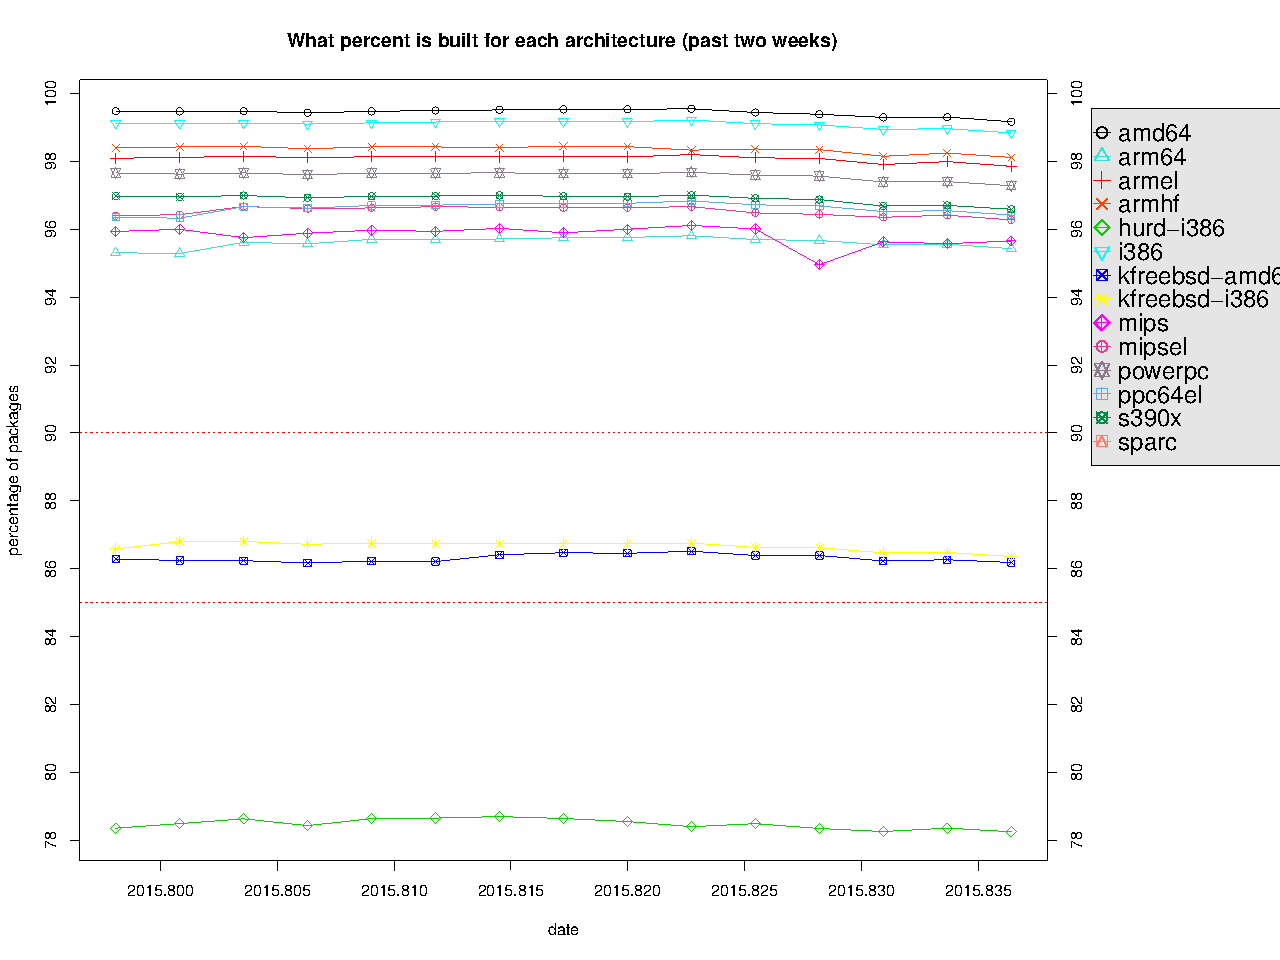
\includegraphics[width=0.7\hsize]{image201511/graph-week-big.png}
%  \end{center}
%
%\end{frame}


\begin{frame}[fragile]
  \frametitle{クロスコンパイル環境}
  \begin{itemize}
  \item Jessie リリース後Debianのクロスコンパイル環境が変わった
  \item 今まではEmdebianから提供されているパッケージを使うか、ユーザ自身でパッケ
ージ化する必要があった。$\leftarrow$ めんどい。

  \item GCCメンテナによりクロスコンパイル用パッケージが提供されるように

  \begin{itemize}
    \item クロス用binutils $\rightarrow$ binutils ソースパッケージ
    \item クロス用libc $\rightarrow$ cross-toolchain-base ソースパッケージ
    \item クロス用GCC $\rightarrow$ gcc-5-cross ソースパッケージ

\begin{commandline}
    $ sudo apt-get install gcc-5-aarch64-linux-gnu
\end{commandline}

  \end{itemize}

  \item リリース対象外のアーキテクチャは未サポート
  \end{itemize}
\end{frame}

\begin{frame}[fragile]
  \frametitle{ユーザランドイメージ}
  \begin{itemize}
  \item インストーラが用意されている \\
	  \url{https://www.debian.org/CD/http-ftp/#stable}
  \item cdebootstrap を使うのが簡単

\begin{commandline}
   $ sudo cdebootstrap --foreign --arch arm64 \
         jessie /tmp/root http://http.debian.net/debian/
\end{commandline}
  \end{itemize}

\end{frame}

\begin{frame}[fragile]
  \frametitle{サポートボード}
  \begin{itemize}
  \item Debian では ARM リファレンスボード(Juno)と X-gene(Applied Micro)のみサポート。
  \item arm64 のボードは値段がクソ高い(10万円以上)上に入手性が悪い。
%FIXME not find image201511/juno.jpg 
%  \begin{center}
%    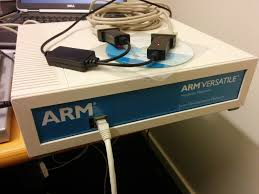
\includegraphics[width=0.5\hsize]{image201511/juno.jpg}
%  \end{center}
  
  \end{itemize}

\end{frame}
\begin{frame}[fragile]
  \frametitle{サポートボード}
  \begin{itemize}
    \item 96boards (Linaro Community Board Program) から入手するのがよさげ。約1万円。
    \begin{center}
    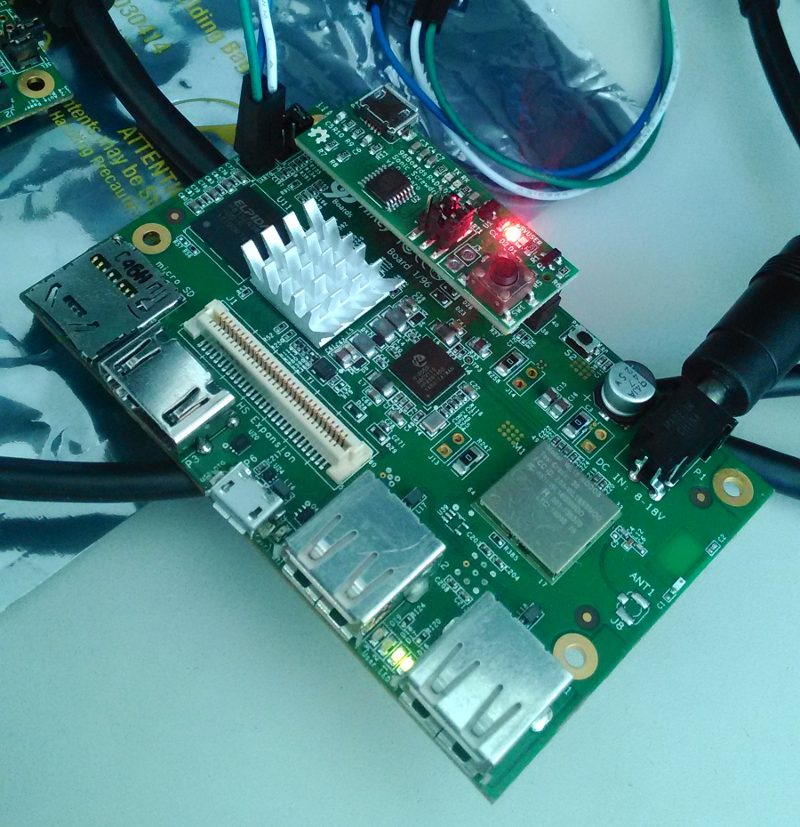
\includegraphics[width=0.3\hsize]{image201511/hikey.png}
    \end{center}
    \begin{itemize}
    \item Linux カーネルパッケージが更新され次第、Debian でもサポートする予定。
    \end{itemize}
  \item QEMU を使って開発することも可能。ただし QEMU 2.0以降。
  \end{itemize}
\end{frame}

\begin{frame}[fragile]
  \frametitle{ベンチマーク}

\begin{table}[htb]
  \begin{tabular}{|l|l|l||l|} \hline
    ベンチマーク  & Raspberry Pi 2 & ODROID-XU4 & Hikey  \\ \hline \hline
    Dhrystone-2 & 1006.6 & 3994.1 & \textcolor{red}{2943.7} \\ \hline
    Double-Precision Whetstone & 361.0 & 1024.9 & \textcolor{red}{680.3} \\ \hline
    Nbench 2.2.3 Integer  & 20.419 & 61.227  & \textcolor{red}{30.803} \\ \hline
    Nbench 2.2.3 FP  & 8.434 & 25.369 & \textcolor{red}{11.889} \\ \hline
  \end{tabular}
\end{table}

\begin{itemize}
\item Raspberry Pi 2: Broadcom BCM2836 900MHz  ARM Cortex-A7 4 core
\item ODROID-XU4: Samsung Exynos5422 Cortex-A15 2Ghz and Cortex-A7 Octa core CPUs
\item Hikey: HiSilicon Kirin 6220 Cortex-A53 1.2Ghz Octa core
\end{itemize}

 \pause

 \begin{center}
 \textcolor{red}{\texttt{ODROID-XU4 > Hikey > Raspberry Pi 2}}
 \end{center}

\end{frame}

%\begin{frame}[fragile]
%  \frametitle{ベンチマーク}
%  \begin{center}
%  \includegraphics[width=0.3\hsize]{image201511/20110809aa_20110809185955.jpg}
%  \end{center}
%\end{frame}

\begin{frame}[fragile]
  \frametitle{ベンチマーク}
  \begin{itemize}
  \item ぶっちゃけ いまのところ ARMv7 の方が速い。
  \item Cortex が遅いという話も。独自コアのSoCはそこそこ速い。
  \item といってもこのまま32bit ARM を使っても2038年問題ががが!
  \item Cortex-A72 に期待。
  \end{itemize}
\end{frame}

\begin{frame}[fragile]
  \frametitle{まとめ}
  \begin{itemize}
  \item Debian では ARM64 が既に使える環境が整っている。
  \item Upstream や 周辺組織との連携も十分。
  \item クロスコンパイル環境もオフィシャルでサポートされるようになり、今まで以上に開発しやすくなっている。
  \item ボードの供給問題がネック。一般向けは 96boards 頼り。
  \item 上記の理由もあり、サポートボードは少ない。今後頑張って増やします。
  \end{itemize}
\end{frame}

%X-gene / Applied Micro X-C1 / 2.4Ghz 8コア 独自 
%Seattle AMD A1100 / 2.0Ghz 8コア A57
%
%etc
%
%64bit になっただけではない
%ECC付きキャッシュ機能などのサーバ向け機能がある


\section{今後の予定}
\begin{frame}[fragile]
\frametitle{今後の予定}

\begin{block}{第104回関西Debian勉強会}
  \begin{itemize}
  \item 日時: 12月
  \item 場所: 未定
  \end{itemize}
\end{block}

\begin{block}{第133回東京エリアDebian勉強会}
  \begin{itemize}
  \item 日時: 10月17日(土)?
  \item 場所: 未定
  \end{itemize}
\end{block}

\end{frame}

\begin{frame}[fragile]
  \frametitle{質問}
  何か質問はありますか?
  \newline \newline \newline \newline

  \begin{itemize}
  \item Contact

    Nobuhiro Iwamatsu
    \begin{itemize}
    \item E-Mail: \href{mailto:iwamatsu@debian.org}{iwamatsu@debian.org}
    \item Twitter: $@$iwamatsu

    \end{itemize}

  \item 資料
    \url{http://tokyodebian.alioth.debian.org/pdf/debianmeetingresume201511-kansai-presentation.pdf}
  \end{itemize}
\end{frame}

\begin{frame}[fragile]
  \frametitle{質問}
  \begin{itemize}
  \item juno.jpg: \url{http://dflund.se/~triad/krad/junoboard/}
  \end{itemize}
\end{frame}


\takahashi[50]{  }

\end{document}
%%% Local Variables:
%%% mode: japanese-latex
%%% TeX-master: t
%%% End:
